\documentclass[12pt,a4paper]{report}
 
\usepackage[utf8]{inputenc}
\usepackage{amsmath,amsthm,amssymb}
\usepackage{braket}
\usepackage{graphicx}

 
\newcommand{\eq}{Eq.}
 
\begin{document}
 

 
\title{Lattice Sinh-Gordon model }
\author{Vincenzo Afferrante, Gianluca Filaci} 
 
\maketitle

\chapter{Introduction} 

Our goal is to simulate  a lattice regularized version of sinh-Gordon model. New results obtained with thermodynamical Bether ansatz give interesting properties, but also many dilemma. In principle, the duality of the theory doesn't work with the mass formula, and there is not a single UV behaviour of the theory, but there can be many values of the charge infinity. A lattice analysis can be helpful to give numerical support to many of this nonperturbative results.

\chapter{Properties of Sinh-Gordon model in the continuum }

The sinh-Gordon model has many remarkable properties. It is integrable, has a unique vacuum and the simplest symmetry $Z_2$: $\phi \to -\phi$. The action that defines it is \begin{equation}
\mathcal{A} = \int d^2x \left\lbrace\dfrac{1}{2 \pi} \sum_\nu (\partial_\nu \phi )^2 + 2 \mu \cosh(b \phi) \right\rbrace 
\end{equation} Due to  integrability 	of the model, the S-matrix is factorizable in 2 particles S-matrix, and it is known analitically \begin{equation}
S(\theta) = \dfrac{\sinh(\theta) -i \sin (\pi \beta)}{\sinh(\theta) +i \sin (\pi \beta) }
\end{equation} Here $\theta$ is the rapidity, and it is related to the energy and the momentum by \begin{equation}
E = m \cosh(\theta) \; ; \; P = m \sinh(\theta)
\end{equation} It is introduced the function $\beta(b)$ defined by \begin{equation}
\beta(b) =  \dfrac{b^2}{8\pi} \dfrac{1}{1+ b^2/8 \pi} \,.
\end{equation} This result is obtained by analytic continuation from an analogous calculation in the sine-Gordon model, valid in the "Coleman bound", namely $b < \sqrt{8\pi}$. It is proven that the theory doesn't develop a mass gap over this bound. 

This formula reveals an interesting property, which is not manifest in the Lagrangian, a duality symmetry given by \begin{equation}
b \to 1/b \; ; \; \beta \to 1- \beta \,.
\end{equation} This transformation doesn't change the position of the zeroes in the S-matrix.


\section{Observables}
Calculations of observable quantities have been made for this model. 
The action used in this calculations is \begin{equation}
\mathcal{A} = \int d^2x  \left\lbrace\dfrac{1}{16 \pi} \sum_\nu (\partial_\nu \phi )^2 + 2 \mu \cosh(b \phi) \right\rbrace 
\end{equation} This action is obtained by $\phi \to 1/ \sqrt{8 \pi} \phi$,
   and by rescaling the coupling accordingly. In this way the Coleman bound is at $b=1$, simplifying the calculations. 
   
   A notable example is obtained for the quantity $e^{a\phi}$, namely
\begin{align}
\braket{e^{a \phi}} =  &\left[ \dfrac{m\Gamma(\frac{1}{2+2b^2}) \Gamma(1+ \frac{b^2}{2+2b^2}) }{4 \sqrt{\pi}}  \right]^{-2 a^2} \times  \\ & \exp{\left\lbrace \int_0^\infty \dfrac{dt}{t} \left[ - \dfrac{\sinh^2(2 a b t)}{2 \sinh(b^2t) \sinh(t)\cosh((1+b^2)t) } + 2 a^2 e^{-2t} \right]  \right\rbrace } \nonumber \,,
\end{align} where \begin{equation}
\label{eq:mass_continuum}
m = \dfrac{4 \sqrt{\pi}}{\Gamma(\frac{1}{2+2b^2})\Gamma(1 +\frac{b^2}{2+2b^2}) } \left[ - \dfrac{\mu \pi \Gamma(1+b^2)}{\Gamma(-b^2)} \right]^{\frac{1}{2+2b^2}} \,.
\end{equation} The last equation gives the renormalized particle mass in terms of the bare parameter $\mu$ and the coupling b. It is remarkable that this formula don't satisfy the duality symmetry, and that the mass goes to zero for $b=1$ (which is equivalent to the Coleman bound, after the rescaling of $1/8\pi$ of the kinetic term).

After the redefinitions $g=b\sqrt{8\pi}$ and $m_0=4b\sqrt{\pi\mu}$, the square of the renormalised mass can be expanded in $g$ as
\begin{align}
\label{eq:exactrenormalisedmassexpansion}
m^2=&m_0^2+\frac{m_0^2g^2}{8\pi}\left(
-\gamma_E+\psi(1/2) +4 \log 2-\log m_0^2
\right)+\notag\\
&+\frac{m_0^2g^4}{384\pi^2}\Big[
3\gamma_E(2+\gamma_E)-\pi^2-24(1+\gamma_E-2\log 2)\log 2+\notag\\
&\qquad\qquad+3\psi(1/2)\left(-2-2\gamma_E+12\log 2+\psi(1/2)\right)+\notag\\
&\qquad\qquad+6\log m_0^2\left(1+\gamma_E-4\log 2-\psi(1/2)\right)+3\log^2m_0^2
\Big]+O(g^6)\,,
\end{align}
where $\gamma_E$ is the Euler–Mascheroni constant and the digamma function $\psi(x)$ is the logarithmic derivative of the gamma function.


\chapter{Lattice setup}

The lattice action (after rescaling the field as $\phi \to 1/\sqrt{8 \pi} \phi $) is \begin{equation}
\mathcal{A} = a^2 \sum_x \left[ \dfrac{N_d}{8 \pi} \phi(x)^2 + \dfrac{1}{8\pi} \sum_\nu \phi(x) \phi(x+ a \nu) +2  \mu \cosh(b\phi(x)) \right] \,.
\end{equation} We can absorb $a^2$ in the dimensioned parameter $\mu$ defining $\hat \mu = a^2 \mu$. We simulate the model using the grid code, based on a HMC algorithm. We will use $a=1$ as usual for the rest of the notes.
The forces for the HMC algorithm are given by \begin{equation}
F(x) = \dfrac{N_d}{4 \pi} \phi(x) + \dfrac{1}{4 \pi} \sum_{\nu}\phi(x+ \nu) + 2 b \mu \sinh(b\phi(x)) \,.
\end{equation}

\chapter{Comparing lattice theory with the continuum }

Simple dimensional analysis show that both the field and the parameter $b$ are dimensionless, while $\mu$ has a dimension 2 in energy. Labelling lattice parameter with an hat, we have $\hat \mu = a^2 \mu$. Naively the continuum is limit is obtained  with $\hat \mu \to 0$. To compare lattice results with the continuum analytic results, we need to find the lines of constant physics.

We can do this using lattice perturbation theory. Calculating the perturbative expansion of the two point function and setting the pole position equal to the mass gives a relation between $ \hat \mu$ and $ b$. This can be checked non-perturbatively doing lattice spectroscopy and checking the value of the physical mass obtained.

The theory has an infinite number of interaction terms \begin{align}
\mathcal{A} &= \sum_x \dfrac{1}{2} \sum_\nu  (\delta_\nu \phi(x))^2 + \dfrac{\hat m_0^2}{g^2} \cosh(g \phi) =\\
  &= \sum_x \left[ N_d \phi(x)^2 +  \sum_\nu \phi(x) \phi(x+\nu) +  \dfrac{\hat m_0^2 }{2}\phi(x)^2 \right. \nonumber \\
  &\left. +   \dfrac{ \hat m_0^2 g^2}{4!} \phi(x)^4 +  \dfrac{ \hat m_0^2 g^4}{6!} \phi(x)^6 + \dots  \right]
\end{align} which leads to an infinite number of Feynman rules for n-point vertex, with n even, namely \begin{equation}
V_n = - \hat m_0^2 g^{n-2} \,.
\end{equation} We chose this action since it doesn't have a factor of the coupling in the bare mass. There is a relation to the $b$ and $\mu$  parameters given by \begin{align}
g = \sqrt{8 \pi} b \; ; \; m_0 = 4 b \sqrt{\pi \mu} \,.
\end{align}
 
  We can expanding the two point function in perturbation theory over powers of the couple $g^2$. In the continuum both the coupling and the field don't renormalize. There is only a multiplicative renormalization of the mass parameter, given by \eqref{eq:mass_continuum}. Setting the two point function \begin{equation}
  D(p^2) = \dfrac{1}{\hat{p^2}+ m^2} +O(\hat{p^2} +m^2)
\end{equation}  for $p^2 \to -m^2$ one obtains \begin{align}
\label{eq:renormalisedmass}
  m^2=&   m_0^2  +\dfrac{1}{2}   m_0^2 g^2 T( m^2)+ \dfrac{1}{8}  m_0^2 g^4 T( m^2)^2 + O(g^6) \\
 = &  m_0^2 (1 + \frac{1}{2}g^2 T( m^2) + \frac{1}{8} g^4 T( m^2)^2 ) + O(g^6 )
 \end{align} We have  the tadpole integral \begin{equation}
 \label{eq:tadpole}
 T(m^2) = \int_{-\pi/a}^{\pi/a} \dfrac{d^2k}{(2 \pi)^2} \dfrac{1}{\hat{k^2} + m^2
  }
 \end{equation} where $\hat{k^2} = \hat{k_x}^2 + \hat{k_y}^2$ and $\hat k = 2/a \sin (ka/2)$. The symmetry factors $1/2$ and $1/8$ are obtained by multiplying the factors $1/4!$ and $1/6!$ of the action by the number of possible connection between vertices and external legs when constructing the tadpole and double tadpole integral.
 It immediately appears that there must be a logarithmic divergence when one substitutes $l_\mu = a k_\mu$ and takes the limit $a\to 0$. 

 
 We can do a similar operation for the coupling, by setting the full four point function with zero external momentum equal to the renormalized coupling constant. We obtain \begin{equation}
 g_R^2 = g^2 +\dfrac{m^2 g^4}{2} T(m^2) + \dfrac{3 m^4 g^4}{2} V(m^2) + O(g^6)
\end{equation} We invert this relation as well, obtaining \begin{equation}
g^2 = g_R^2\left[1- \left(\dfrac{3m^2}{2}T(m^2) - \dfrac{3m^4}{2}V(m^2) \right)g_R^2 \right] + O(g_R^4)
\end{equation} 
 We can substitute $\hat m_0^2$ with $\hat m^2$ in the integrals with an error of order $g^6$. We invert the series \begin{equation}
  m_0^2 =  m^2\left[1 - \frac{1}{2}g^2 T(  m^2) + \left( \frac{1}{8}  T(m^2)^2+ \dfrac{3 m^2}{4}(T^2 +m^2VT) \right) g^4  \right] + O( g^6 ) \,.
 \end{equation} This formula gives us, given a physical value of the mass $m$, the bare parameter $m_0$ for a fixed value of the lattice spacing $a$. We need to evaluate the tadpole and the vertex correction integrals.
  
 \section{Evaluation of the integrals}
 
 We substitute $l_\mu = a k_\mu$ in \eqref{eq:tadpole} obtaining \begin{equation}
 T( m^2) =  \int_{-\pi}^\pi \dfrac{d^2l}{(2 \pi)^2}\dfrac{1}{\hat l^2 + a^2m^2} =  I_1(a^2 m^2) \,.
 \end{equation} The integral has infrared divergencies for $a \to 0$. We define \begin{equation}
 I_n(\xi^2) = \int_{-\pi}^\pi \dfrac{d^2l}{(2 \pi)^2}\dfrac{1}{(\hat l^2 + \xi^2)^n}
\end{equation}  We can evaluate numerically the value of $I_1$ for $a\to 0$ only dividing the integral in two parts, one within a small radius $\rho$, and the other outside.
 We obtain:
 \begin{align}
 I_1(\xi^2) &= \int_{|l|< \rho} \dfrac{d^2l}{(2 \pi)^2} \dfrac{1}{l^2 + \xi^2} +\int_{|l|> \rho} \dfrac{d^2l}{(2 \pi)^2} \dfrac{1}{\hat l^2 + \xi^2}  \\
 &= \dfrac{1}{4 \pi} \dfrac{\xi^2}{\rho^2} - \dfrac{1}{4 \pi} \ln \left( \dfrac{\xi^2}{\rho^2}\right) + \int_{|l|> \rho} \dfrac{d^2l}{(2 \pi)^2} \dfrac{1}{\hat l^2 } - \xi^2 \int_{|l|> \rho} \dfrac{d^2l}{(2 \pi)^2} \dfrac{1}{(\hat l^2)^2}  +O(\xi^4) \nonumber \\
 &= Z_0 -\xi^2 C_0 -\dfrac{1}{4 \pi} \ln(\xi^2) ,. \nonumber
 \end{align} We have expanded both parts in powers of $a^2$. We defined $\xi^2 = a^2 m^2$ and we introduced the quantities
\begin{align}
Z_0 &= \lim_{\rho \to 0} \int_{|l|> \rho}  \dfrac{d^2l}{(2 \pi)^2} \dfrac{1}{\hat l^2 } + \dfrac{1}{4 \pi} \log(\rho^2)=0.275794 \,, \\
C_0 &= \lim_{\rho \to 0}  \int_{|l|> \rho}  \dfrac{d^2l}{(2 \pi)^2} \dfrac{1}{(\hat l^2)^2 } - \dfrac{1}{4 \pi \rho^2} \,.
\end{align} In this case the quantities $C_0$ is ininfluent for $a\to 0$, so we have the result \begin{equation}
I(a^2 m^2)= Z_0 - \dfrac{1}{4 \pi} \ln(a^2m^2) \,.
\end{equation} For the evaluation of the vertex corrections, we note that \begin{equation}
V(m^2) = \int_{-\pi/a}^{\pi/a} \dfrac{d^2k}{(2 \pi)^2}\dfrac{1}{(\hat k^2 + m^2)^2} = a^2 I_2(a^2 m^2) \,.
\end{equation} We use the relation \begin{equation}
I_2(\xi^2) = - \dfrac{d}{d\xi^2} I_1(\xi^2) = C_0 + \dfrac{1}{4 \pi \xi^2} + O(\xi^2) \,.
\end{equation} We have the final result: \begin{align}
  m_0^2 &=  m^2\left[1 - \frac{1}{2}g^2 I_1( a^2 m^2) + \left(\frac{1 + 6m^2}{8} I_1(a^2m^2) + \dfrac{3m^4a^2}{4}I_1(a^2m^2)I_2(a^2m^2)  \right) g^4 \right] + O( g^6 ) \\
g^2 &= g_R^2\left[1- \left( \dfrac{m^2}{2}I_1(a^2 m^2) - \dfrac{3m^4a^2}{2} I_2(a^2m^2) \right)g_R^2 \right] + O(g_R^6) \,.
\end{align}
 
\paragraph{Comment}
We have shown that $T(m^2)=Z_0-\frac{1}{4\pi}\log a^2m^2 + O(a^4m^4)$.
From \eq~\eqref{eq:renormalisedmass}, this implies that the coefficients of $\log a^2m^2$ at $O(g^2)$ and $(\log a^2m^2)^2$ at $O(g^4)$ match those in \eq~\eqref{eq:exactrenormalisedmassexpansion}.
 
\chapter{Mass scaling on the lattice} 

We are interested in verifying the assumptions given by the mass formula \eqref{eq:mass_continuum} for  mass values we can obtain with lattice with our setup. We want to do this motivated by the comment of the last section. Since the coefficients in front of the logarithm mathches, we want to use the result relative to the resummation of the logarithm at every order, which gives the $\mu^{1/(2+2b^2)}$ behaviour. The coefficient in front of that will be a result of the lattice regularization, and will be affected heavily by lattice artefacts.

We used as spectroscopical operator the time sliced field \begin{equation}
O(t) = \sum_x \phi(t,x)
\end{equation} We chose one direction as the temporal one, and we summed over the other. Since the theory has no bound states, we expect that there shouldn't be contaminations in the first time slices, and also that the majority of the signal should be in the first time slices. Given the correlation function \begin{equation}
C(t) = \sum_{t'=0}^{N_t-1} O(t') (t'+t) 
\end{equation} we expect the following behaviour in this region \begin{equation}
C(t) \approx e^{-m_{eff} t} \,.
\end{equation} We can extract the mass as \begin{equation}
m_{eff}(t+0.5) = \log \dfrac{C(t)}{C(t+1)} \,.
\end{equation}


Inspired by \eqref{eq:mass_continuum}, we want to observe a behaviour given by \begin{equation}
\label{eq:lattice_mass_scaling}
m_{eff}= f(b) \, \mu^\alpha
\end{equation} with $f(b)$  an unknown function of the parameter "b", really sensible to lattice regularization artefacts, while we expect $\alpha$ to be close to the value obtained in the continuum, namely $1/(2+2b^2)$. 

For a fixed beta we proceeded to fit the mass obtained with spectroscopy for various values of $\mu$.


The green line represent the fit with the $\alpha$ parameter free to vary, while the red one fixes $\alpha$ to be the theoretical value predicted in \eqref{eq:mass_continuum}.

We expect the results to be close to the continuum limit for small values of the effective mass, since, given a fixed measured value of the physical mass $m^*$ , it is related to the lattice mass simply by \begin{equation}
a m^* =  \, \hat m_{lat}
\end{equation} with $a$ being the lattice spacing. We used  values of $m_lat$ between $0.001$ and $1$, we believe are reasonably close to the continuum limit in this region. Lower values of the effective mass results in a theory with a really slow growing potential, and the numerical algorhithms for these cases generates very correlated configurations. Higher values of the effective mass increase lattice artefacts considerably, and this can invalidate our assumption of the behaviour, so they will not be considered as well.
\begin{figure}
\label{fig:mass_scaling_b0.1}
\centering
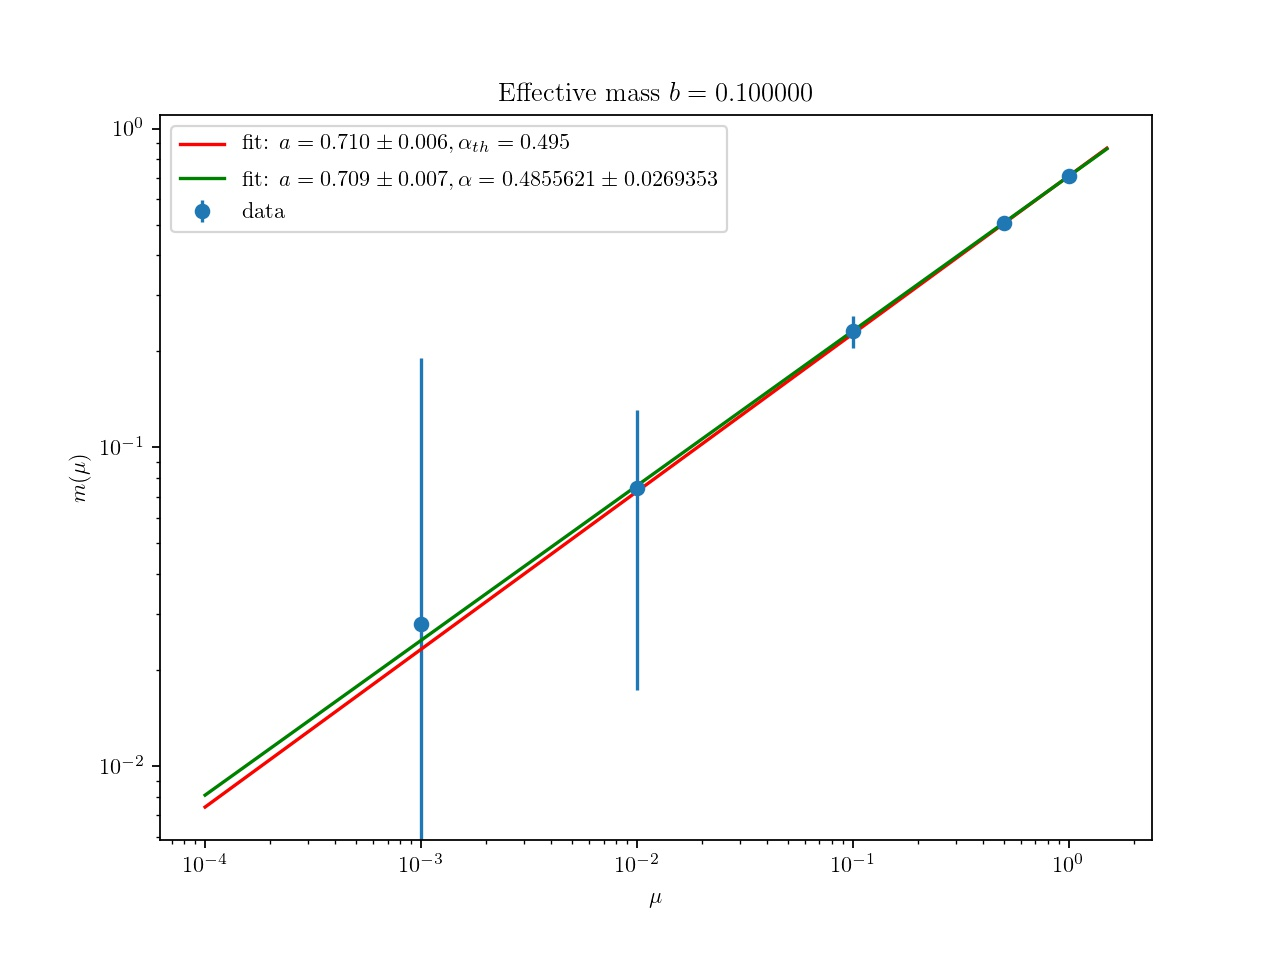
\includegraphics[width=1.0\textwidth]{b0_1}
\caption{Value of the masses obtained for $b=0.1$ and 
$\mu = [0.001,0.01,0.1,0.5,1]$. The $\chi^2$ for the two fit are 0.031159556043223686 and 0.0005302957212052317, for the case with fixed $\alpha = 1/(2+2b^2)$ and with $\alpha$ free, respectively.}
\end{figure}

In figure \ref{fig:mass_scaling_b0.1} we show the results for $b=0.1$. We obtained \begin{equation}
f = 0.710 \pm 0.006
\end{equation} with $\alpha_{th}$ fixed at $0.495$ and \begin{equation}
f= 0.709 \pm 0.007 \,,\, \alpha = 0.486 \pm 0.03
\end{equation} with $\alpha$ free.

\begin{figure}
\label{fig:mass_scaling_b0.2}
\centering
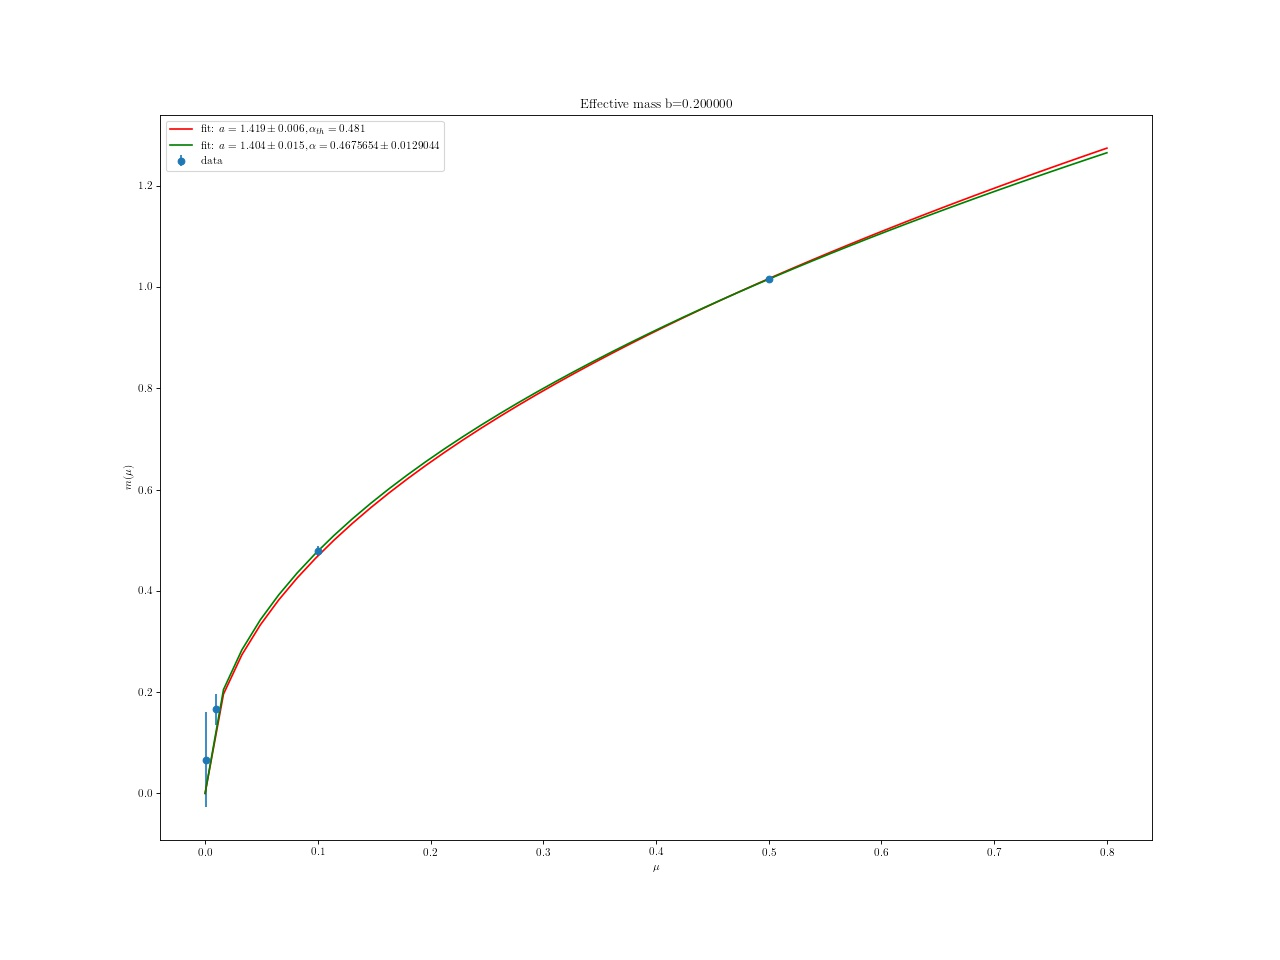
\includegraphics[width=1.0\textwidth]{b0_2}
\caption{Value of the masses obtained for $b=0.2$ and 
$\mu = [0.001,0.01,0.1,0.5]$. The $\chi^2$ for the two fit are 0.3488364928360326 and 0.011429390512562691, for the case with fixed $\alpha = 1/(2+2b^2)$ and with $\alpha$ free, respectively.}
\end{figure}

In figure \ref{fig:mass_scaling_b0.2} we show the results for $b=0.2$. We obtained \begin{equation}
f = 1.419 \pm 0.006
\end{equation} with $\alpha_{th}$ fixed at $0.481$ and \begin{equation}
f= 1.404 \pm 0.015 \,,\, \alpha = 0.47 \pm 0.01
\end{equation} with $\alpha$ free.
 
\end{document}